\documentclass[11pt]{article}
\usepackage[margin=1in]{geometry}
\usepackage{amsmath,amssymb}
\usepackage{graphicx}
\usepackage{booktabs}
\usepackage{xcolor}
\usepackage{caption}
\usepackage{microtype}
\usepackage{enumitem}
\usepackage{hyperref}
\usepackage{titlesec}

\setlength{\parskip}{1pt}
\setlength{\parindent}{0pt}
\titlespacing*{\section}{0pt}{8pt}{3pt}
\titlespacing*{\subsection}{0pt}{6pt}{2pt}
\titleformat{\section}{\normalfont\bfseries}{\thesection.}{0.4em}{}
\titleformat{\subsection}{\normalfont\bfseries\itshape}{\thesubsection.}{0.4em}{}
\renewcommand{\thesection}{\arabic{section}}
\captionsetup{font=small,skip=3pt,labelfont=bf}
\setlist[itemize]{leftmargin=*,topsep=2pt,itemsep=1pt,parsep=0pt}
\setlist[enumerate]{leftmargin=*,topsep=2pt,itemsep=1pt,parsep=0pt}

\newcommand{\code}[1]{\texttt{#1}}
\graphicspath{{figs/}}
\hypersetup{colorlinks=true,linkcolor=blue,citecolor=blue,urlcolor=blue}

\begin{document}

\begin{center}
{\Large\bfseries GPU-Accelerated TEBD for the 1D Transverse-Field Ising Model}\\[4pt]
{\large Final Report, CME 213: Parallel Computing with CUDA, MPI and OpenMP}\\[3pt]
{\normalsize Hercy Shen, Chiling Han, Xin Wei\quad|\quad June 8, 2026}
\end{center}



%% -------------------------------------------------------------------------
\section{Project description}

We simulate the \textbf{real-time quench dynamics} of the one-dimensional transverse-field Ising model (TFIM), a canonical quantum many-body system, with Hamiltonian
\begin{equation}
  H = -J\sum_i \sigma^x_i\sigma^x_{i+1} \;-\; g\sum_i \sigma^z_i .
\end{equation}
A chain of $L$ spin-$\tfrac{1}{2}$ sites lives in a Hilbert space of dimension $2^L$, so storing the wavefunction exactly is impossible beyond $L\approx30$. What makes this tractable is that low-energy and short-time states of 1D local Hamiltonians stay weakly entangled, so they compress into a \textit{Matrix Product State (MPS)}: the $2^L$ amplitudes factor into $L$ small rank-3 tensors connected by \emph{bond} indices of dimension $\chi$. The MPS stores only $O(L\chi^2 d)$ numbers ($d=2$), where $\chi$ grows with the entanglement across each cut.


\textbf{Computation.} We evolve the state with \textit{Time-Evolving Block Decimation
(TEBD)}: the propagator $e^{-iHt}$ is Suzuki--Trotter split into nearest-neighbour two-site gates $U_b=e^{-i\,\Delta t\,H_b}$, and each Trotter step applies $L-1$ gates. Applying one gate is one small complex SVD that re-compresses the two-site tensor back to bond dimension $\chi$; this SVD takes $>99.6\%$ of GPU kernel time and is the target of all parallel work here.

\begin{itemize}
\item \textbf{Inputs:} chain length $L$; couplings $(J,g)$; an initial product state;   Trotter step $dt$; number of steps $N$; max bond dimension $\chi_{\max}$.
\item \textbf{Outputs:} mean field magnetizations $\langle\sigma^z_i\rangle$,  $\langle\sigma^x_i\rangle$, two-point correlations $\langle\sigma^x_i\sigma^x_j\rangle$, the bipartite von-Neumann entanglement entropy, and the bond-dimension profile $\chi(t)$.
\item \textbf{Assumptions:} open boundary conditions, local dimension $d=2$.
\end{itemize}

\textbf{Why parallelism.} Entanglement grows under a quench, so $\chi(t)$ climbs over time (Fig.~\ref{fig:summary}) until it saturates $\chi_{\max}$. Each bond update requires a small dense SVD whose cost scales roughly as $O(\chi^3)$, so doubling the effective bond dimension gives an $8\times$ increase in work.
% On a single GPU, each bond update runs as device kernels: our CUDA kernels handle the gate contraction, layout conversion, and reconstruction of the MPS tensors around the SVD, while cuSOLVER performs the SVD in the production path.

Across GPUs we use task parallelism: each MPI rank owns one GPU and runs independent TEBD evolutions for different $(J,g)$ points -- a natural fit for the parameter sweep.

%% -------------------------------------------------------------------------
\section{Algorithms and state of the art}

\textbf{Core algorithm.} We implement TEBD on a \textit{right-canonical MPS} in Vidal form. The two-site update is:
(1) contract the gate with the two-site tensor;
(2) SVD the reshaped $(\chi_L d)\times(d\chi_R)$ matrix;
(3) truncate to the largest $\chi_{\max}$ singular values and renormalize;
(4) restore MPS form.

\textbf{State of the art.}
Mature libraries (\textit{TeNPy}, \textit{ITensor}, \textit{quimb}, \textit{TensorNetwork}) are CPU/Python-centric and general; on GPUs, NVIDIA's \textit{cuTensorNet} (cuQuantum) offers library-level batched contraction and SVD. The algorithmic variants relevant to our problem are the SVD engine, the time integrator (Trotter--Suzuki), and the parallel decomposition.

\textbf{Our choice and how it compares.} We do not try to beat cuTensorNet on throughput; instead we build an instrumented TEBD that times each stage separately, so we can attribute time to gate contraction, SVD, truncation, and PCIe traffic rather than let a library hide it.
% For the SVD we chose \textit{one-sided Jacobi}: at our matrix sizes ($2\chi \lesssim 256$) it converges in 5 - 10 sweeps and avoids the QR preprocessing that \code{gesvd} only amortizes on large matrices. We implement it two ways: a complete from-scratch CUDA one-sided Jacobi (our computationally intensive hand-written kernel, \code{jacobi\_sweep}/\code{jacobi\_finish}) and the production path through cuSOLVER's \code{gesvdj} as a tuned-library baseline; running both quantifies the gap to the standard library directly (\S7).

%% -------------------------------------------------------------------------
\section{Parallelization strategy (CUDA + MPI)}\label{sec:parallel}

\subsection{The central difficulty and our decomposition}

A single TEBD chain has \textit{limited spatial parallelism}. Within one Trotter sub-step the even bonds $\{0,2,4,\dots\}$ and odd bonds $\{1,3,5,\dots\}$ touch disjoint tensors and are independent ($\sim(L-1)/2$-way), but the even and odd sub-steps are \emph{sequential}, and a spatial decomposition that splits the chain across ranks would require one MPI round-trip per sub-step to exchange the boundary Schmidt spectrum. We benchmark up to $L=80$ and found that the per-step compute is far too small to hide that latency.

We therefore use \textit{task parallelism}: each MPI rank owns one GPU and runs complete, independent TEBD evolutions for a set of $(J,g)$ points in the phase diagram, with zero in-loop communication. We rejected two alternatives: (a) spatial chain decomposition, infeasible at small $L$ due to per-sub-step synchronization; (b) replicated-parameter plus distributed chain, which needs per-bond MPI barriers.

\subsection{Single-GPU bond-update pipeline}

The bond update runs as a five-stage device pipeline -- gate contraction (gate staged in \textbf{shared memory}), a \textbf{coalesced} row$\to$col relayout, the SVD ($>99.6\%$ of kernel time, \S\ref{sec:bench}), and two Vidal-restore steps (full kernel list in Appendix~\ref{app:pipeline}).

\subsection{Persistent device-resident MPS and streams}

\begin{itemize}
\item \textbf{Persistent device MPS.} All tensors and Schmidt spectra stay device-resident for the whole evolution, and the buffers are pre-allocated once, so nothing is allocated during the evolution itself.
\item \textbf{Streams within a sub-step.} A sub-step can run several workspaces on independent CUDA streams. But truncation needs a host sync mid-bond to read the singular values, which serializes the bonds, so the measured stream speedup is negligible (Table~\ref{tab:gpu}).
\end{itemize}

\subsection{MPI decomposition and communication pattern}

Each rank calls \code{cudaSetDevice(rank \% n\_gpus)}, builds its $(J,g)$ points locally (no scatter), and runs independent evolutions; the TEBD loop contains no MPI calls. Only at the end does rank 0 collect results: an \code{MPI\_Gather} of per-rank record counts, then an \code{MPI\_Gatherv} of the variable-length records.

%% -------------------------------------------------------------------------
\section{Performance model}

The performance model has four parts, each with a falsifiable prediction.

\textbf{(a) Per-bond compute and the latency/compute crossover.} The dominant cost is the SVD of a $2\chi_a\times2\chi_a$ complex matrix. One-sided Jacobi does $O(\chi_a^3)$ flops per sweep over $\sim5$--$10$ sweeps, plus a fixed overhead $t_0$ per bond, giving $T_\text{step}(L,\chi_a)\approx(L-1)(t_0 + c\,\chi_a^3)$. \textbf{Predictions:} (i) when $c\chi_a^3\ll t_0$ the code is \textbf{latency-bound}: $T$ is linear in $L$ and flat in $\chi_{\max}$; (ii) when $c\chi_a^3\gg t_0$ it becomes \textbf{work-dominated}: $T\propto\chi_a^3$. Our runs sit in branch (i) (\S\ref{sec:bottleneck}).

\textbf{(b) Roofline / arithmetic intensity.} Each Jacobi sweep does $O(\chi_a^3)$ flops on an $O(\chi_a^2)$-word matrix that fits in L2, so intensity $I=O(\chi_a)$ grows with $\chi_a$ and the matrix is cache-resident. \textbf{Prediction:} the SVD is never bandwidth-bound; at the small realized $\chi_a$ the limiter is kernel-launch and dispatch latency, not bandwidth or peak compute, and the compute roof is reached only at $\chi_a$ far beyond our range.

\textbf{(c) Communication model.} The only message is the final \code{Gatherv} of $\lesssim10$ KB.
\textbf{Prediction:} communication fraction $<10^{-4}$, invisible in a profiler.

\textbf{(d) Parallel efficiency (task-parallel load balance).} With $P$ ranks and per-pair costs $t_i$, efficiency is $E=\bigl(\sum_i t_i\bigr)/\bigl(P\,\max_r\sum_{i\in r}t_i\bigr)$. Pair cost rises steeply with $J$: more entanglement means larger $\chi_a$, and the SVD work grows as $O(\chi_a^3)$.
% Round-robin prediction: $E\approx80\%$ at $P=4$.

%% -------------------------------------------------------------------------
\section{Benchmarking and instrumentation}\label{sec:bench}

\textbf{Instrumentation.} Per-stage GPU time measured with \textit{CUDA events} (\code{bench\_breakdown}); full-step wall time via host timers (\code{bench\_gpu});
SVD-engine comparison via \code{bench\_svd}; end-to-end timelines with \textit{Nsight Systems} (\code{nsys profile}), single-GPU and under \code{mpirun -n 4}.

\smallskip
\noindent\textbf{Single-GPU full-step timing} (\code{bench\_gpu}, $L=20$, 20 steps, \code{gpu-turing}):

\smallskip
\begin{center}\begin{tabular}{rrrrrr}
\toprule
$\chi_{\max}$ & CPU (s) & M3 GPU (s) & Persistent (s) & Streamed (s) & CPU/Persistent \\
\midrule
 16 & 2.049  & 5.372  & 5.180  & 5.183  & 0.40 \\
 32 & 9.601  & 13.196 & 12.992 & 13.064 & 0.74 \\
 48 & 20.073 & 17.428 & 17.075 & 17.079 & 1.18 \\
 64 & 24.099 & 18.250 & 17.709 & 17.745 & 1.36 \\
 96 & 24.484 & 18.269 & 17.722 & 17.854 & 1.38 \\
128 & 24.533 & 18.334 & 17.848 & 17.853 & 1.37 \\
\bottomrule
\end{tabular}
\end{center}

\smallskip
\captionof{table}{GPU overtakes CPU at $\chi_{\max}\ge48$; persistent MPS is 1--3\% faster than M3 host-staging; four streams add nothing.}\label{tab:gpu}

\noindent A per-kernel breakdown (\code{bench\_breakdown} / Nsight \code{cuda\_gpu\_kern\_sum}) confirms the SVD dominates: cuSOLVER Jacobi is $>99.6\%$ of GPU kernel time, all our custom kernels together $<0.4\%$, and MPI $<0.01\%$ (Table~\ref{tab:breakdown}).

\smallskip
\textbf{Model vs.\ measurement.} The crossover study (Fig.~\ref{fig:crossover}) confirms prediction (a): at TFIM-realized $\chi_a\approx41$ the GPU is latency-bound (flat across $\chi_{\max}=64$--128 in Table~\ref{tab:gpu}), crossing the CPU near $\chi\approx96$
and reaching $\sim5\times$ at $\chi=128$. Nsight confirms model (c): no MPI call appears in the timeline.

%% -------------------------------------------------------------------------
\section{Bottleneck analysis}\label{sec:bottleneck}

The bottleneck has three parts, each tied to hardware.

\begin{itemize}
\item \textbf{Not memory-bound.} The SVD is $>99.6\%$ of kernel time (Table~\ref{tab:breakdown}), and roofline rules out bandwidth: the L2-resident $2\chi_a\times2\chi_a$ matrix has intensity $\sim95\times$ past the ridge at $\chi_a=64$. But that only rules out bandwidth -- it does not show the kernel reaches the compute roof.

\item \textbf{Latency-bound at the realized sizes.} Entanglement fixes the realized $\chi_a\approx41$ ($\le64$ across the sweep), too small to saturate the SMs. The GPU/CPU ratio in Table~\ref{tab:gpu} confirms this: the GPU loses at small $\chi_{\max}$ (launch overhead $t_0$ dominates), then wins only $\sim1.4\times$ and plateaus as $\chi_a$ saturates -- a compute-bound kernel would instead keep speeding up.

\item \textbf{Multi-GPU: load imbalance, not communication.} Computation is $>99\%$ of wall time (\code{Gatherv} $<0.01\%$), so the distributed bottleneck is \textbf{load imbalance}: round-robin hands one rank the four hardest ($J=2.0$) pairs, $\sim2.2\times$ the cheapest, giving the $\sim19\%$ gap at $P=4$ (\S\ref{sec:scaling}, Fig.~\ref{fig:phase}).
\end{itemize}

\textbf{Custom-kernel profiling (Nsight Compute).} \code{ncu} on our hand-written Jacobi kernel (Appendix~\ref{app:ncu}) shows the same story at the kernel level: a single $128$-thread block leaves 1 of 72 SMs active ($\approx99.8\%$ idle) and stalls $41.6\%$ of the time at per-rotation \code{\_\_syncthreads} barriers -- under-decomposed and latency-bound, not compute- or memory-bound. cuSOLVER keeps far more of the device busy ($1.2$--$2.2\times$ faster, Table~\ref{tab:svd}). This is the same shortage of per-chain parallelism behind our task-parallel design (\S\ref{sec:parallel}): even batching the $\sim(L-1)/2$ bonds would not fill 72 SMs at $L\le80$.

%% -------------------------------------------------------------------------
\section{Algorithmic variants and their effect on performance}

We explored four variants; each shifts the bottleneck differently.

\begin{enumerate}
\item \textbf{Host-staging (M3) $\to$ persistent device MPS.} Eliminating per-bond H2D/D2H cuts PCIe traffic from tens of MB to $\sim0.2$ MB for a steady 1--3\% speedup (Table~\ref{tab:gpu}), small because the SVD dominates.

\item \textbf{Single stream $\to$ 4 streams.} Negligible (Table~\ref{tab:gpu}, Fig.~\ref{fig:gputiming}). The model predicted it; profiling showed why: host-side truncation serializes bonds.

\item \textbf{cuSOLVER \code{gesvdj} vs.\ custom one-sided Jacobi SVD.} Our hand-written Jacobi kernel is \textbf{1.2--2.2$\times$ slower} than cuSOLVER and agrees to $\lesssim10^{-12}$ (Table~\ref{tab:svd}, Fig.~\ref{fig:svd}). Both paths plateau once $\chi_{\max}$ exceeds the realized $\chi_a\approx41$--64 (cuSOLVER time changes $<1\%$ from $\chi_{\max}=64$ to 256), a direct consequence of the latency-bound regime: SVD matrix size is set by $\chi_a$, not $\chi_{\max}$.

\item \textbf{Trotter order (1/2/4).} Higher order trades more gates per step for $O(dt^p)$ accuracy; order 4 (Forest--Ruth) reaches the ED-validation floor ($\sim10^{-6}$) at larger $dt$.
\end{enumerate}

\smallskip
\begin{center}\begin{tabular}{rrrrl}
\toprule
$\chi_{\max}$ & cuSOLVER (s) & Custom Jacobi (s) & Ratio & max $|\Delta\sigma|$ \\
\midrule
 16 &  7.110 &  8.184 & 0.869 & $4.74\times10^{-14}$ \\
 32 & 17.352 & 27.089 & 0.641 & $5.84\times10^{-13}$ \\
 48 & 22.688 & 46.056 & 0.493 & $9.96\times10^{-13}$ \\
 64 & 23.751 & 52.160 & 0.455 & $1.00\times10^{-12}$ \\
128 & 23.754 & 52.208 & 0.455 & $1.00\times10^{-12}$ \\
256 & 23.985 & 52.435 & 0.457 & $1.00\times10^{-12}$ \\
\bottomrule
\end{tabular}
\end{center}

\smallskip
\captionof{table}{\code{bench\_svd}: cuSOLVER vs.\ custom Jacobi, $L=20$, 20 steps. Both paths
plateau above $\chi_{\max}=64$;
% the wide-matrix adjoint fix reduced error from $O(10^{-1})$ to $\lesssim10^{-12}$.
}\label{tab:svd}

%% -------------------------------------------------------------------------
\section{Scalability analysis}\label{sec:scaling}

We study scaling of the task-parallel sweep on \code{gpu-turing}, using total rank
wall time $T(P)=\max_r\sum_{i\in r}t_i$.

\smallskip
\begin{center}\begin{tabular}{lrrrrl}
\toprule
Mode & Ranks & Pairs/rank & Time (s) & Speedup & Efficiency \\
\midrule
strong & 1 & 16 & 321.6 & 1.00 & 100\% \\
strong & 2 &  8 & 184.3 & 1.75 &  87\% \\
strong & 4 &  4 &  99.1 & 3.24 &  81\% \\
weak   & 1 &  4 &  17.1 & n/a  & 100\% \\
weak   & 2 &  4 &  59.1 & n/a  &  29\% \\
weak   & 4 &  4 & 103.5 & n/a  &  17\% \\
\bottomrule
\end{tabular}
\end{center}

\smallskip
\captionof{table}{MPI strong and weak scaling. Strong speedup relative to $P=1$ wall time (321.6 s).}\label{tab:scaling}

\textbf{Strong scaling.} Speedup reaches $3.24\times$ at $P=4$ (81\% efficiency, Fig.~\ref{fig:scaling}). The 19\% loss is exactly the load imbalance the model predicted: round-robin hands rank 3 the four $J=2.0$ pairs (highest entanglement), which run $\sim2.2\times$ longer than rank 0's cheap $J=0.25$ pairs. Communication is $<0.01\%$.

\textbf{Weak scaling.} Efficiency falls sharply (29\% at $P=2$, 17\% at $P=4$), but this is \emph{not} a communication or synchronization failure. The weak mode hands each added rank \emph{higher-$J$} pairs, which are intrinsically more expensive ($2$--$6\times$ the cost of the $P=1$ pairs). True constant-work weak scaling would require balancing by \emph{estimated entanglement} rather than pair count.

\begin{figure}[ht]
  \centering
  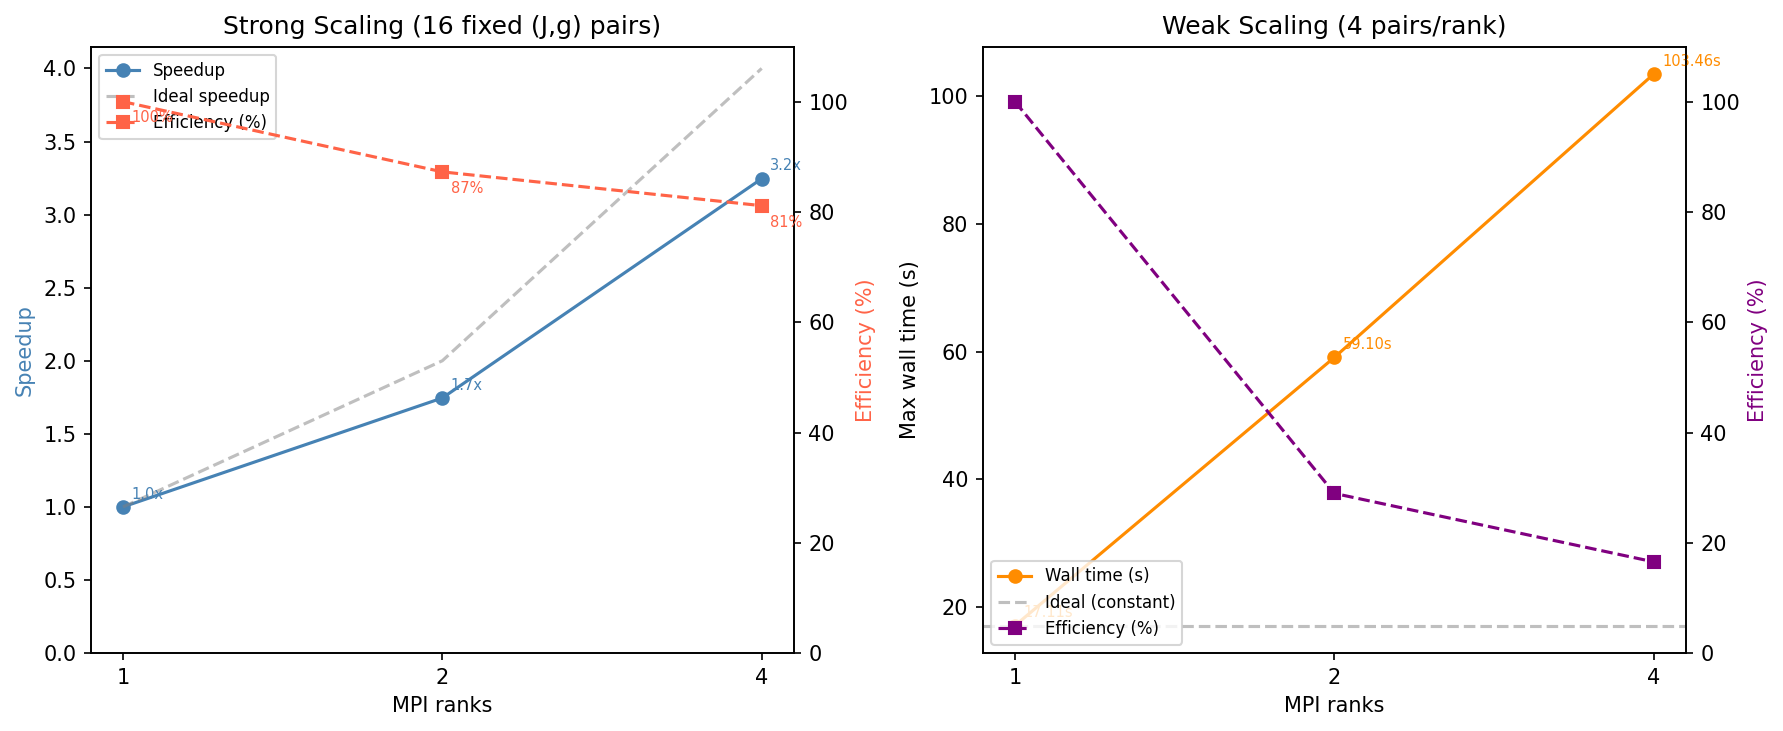
\includegraphics[width=0.82\linewidth]{scaling_m4.png}
  \caption{Strong-scaling speedup (left) and weak-scaling wall time (right) (companion to Table~\ref{tab:scaling}).}
  \label{fig:scaling}
\end{figure}

\textbf{Phase-diagram structure.} Figure~\ref{fig:phase} shows the end-of-evolution mid-chain entropy and realized $\chi_a$ across the $4\times4$ grid: entropy peaks near the critical point ($J\approx g$) and saturates $\chi_{\max}=64$ at most high-$J$ points, while the paramagnetic corner reaches only $\chi_a\approx21$--45. This 2--6$\times$ spread in $\chi_a$ sets the per-pair SVD cost and explains the load-imbalance gap.

\begin{figure}[ht]
  \centering
  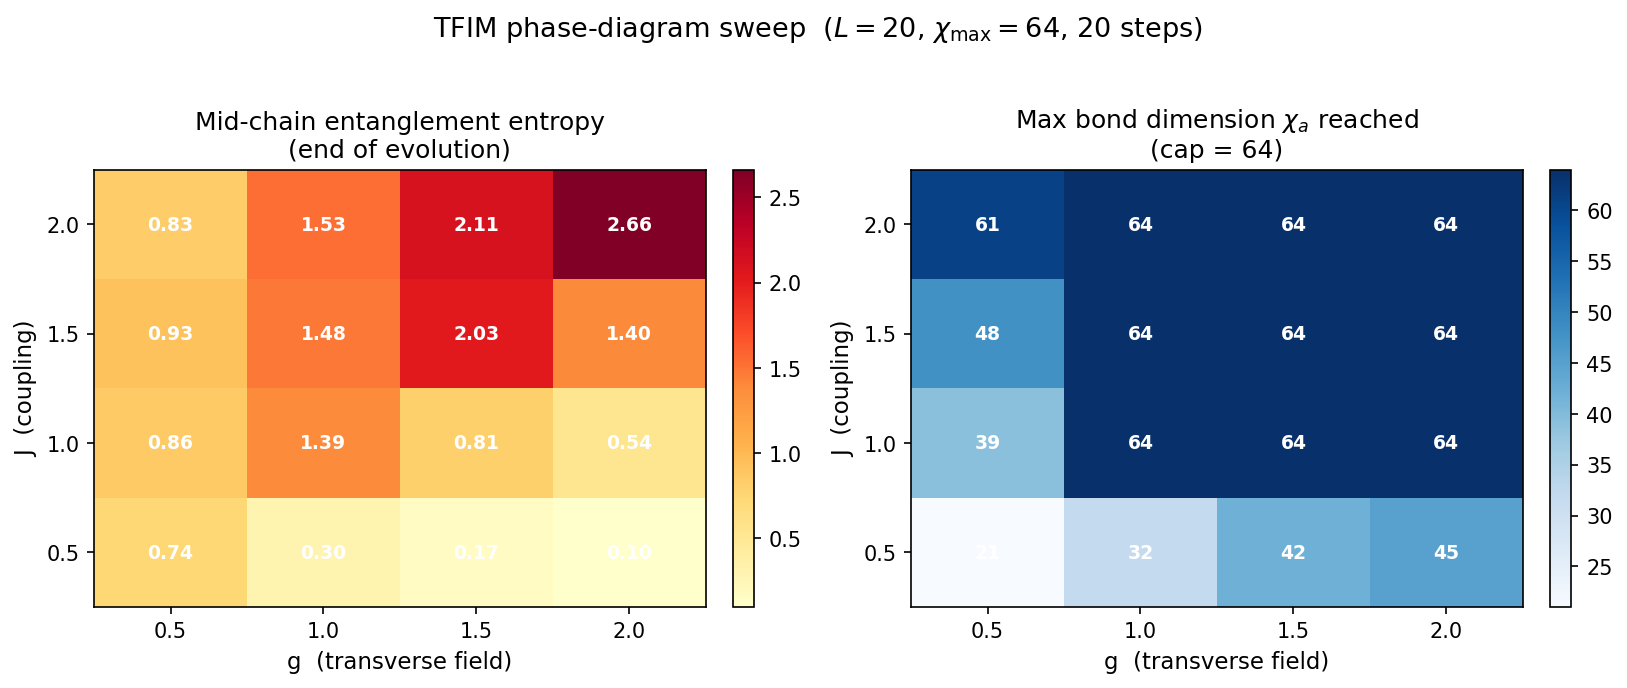
\includegraphics[width=0.9\linewidth]{phase_heatmap.png}
  \caption{Left: final mid-chain entropy $S_\text{mid}$. Right: max realized bond dimension $\chi_a$. High-$J$ points saturate $\chi_{\max}=64$ and dominate runtime; the paramagnetic corner (small $J$, large $g$) is cheap.}
  \label{fig:phase}
\end{figure}

% \textbf{Observables over the phase diagram.} The sweep also collects GPU-computed $\langle\sigma^z_i\rangle$, $\langle\sigma^x_i\rangle$, and $\langle\sigma^x_i\sigma^x_j\rangle$ for every pair (Fig.~\ref{fig:obs}). $\langle\sigma^x_i\rangle$ is zero by parity ($H$ commutes with $\Pi=\bigotimes\sigma^z_i$, under which $\sigma^x_i\to-\sigma^x_i$), and the ferromagnetic corner (large $J$, small $g$) shows the largest NN correlations and smallest $|\langle\sigma^z_i\rangle|$, as expected.

%% -------------------------------------------------------------------------
\section{Correctness and verification}\label{sec:correct}

We verify correctness at four independent levels.
\begin{enumerate}
\item \textbf{Unit tests.} 54 Google Test cases over 6 binaries cover the tensor and hand-written linear-algebra ops, observables, the TFI model, and TEBD invariants (norm, $S^z$, entropy growth, Trotter convergence), all passing at $10^{-12}$ (exact) / $10^{-10}$ (SVD-dependent).

\item \textbf{Exact-diagonalization oracle.} Against a full $2^L\times2^L$ evolution at $L=8$ (order 4, $\chi_{\max}=64$), TEBD reaches $\sim5\times10^{-6}$ max error in observables and entropy with fidelity loss $4.3\times10^{-11}$, dominated by the $O(dt^4)$ Trotter floor (Fig.~\ref{fig:validate}).

\item \textbf{CPU$\leftrightarrow$GPU agreement.} GPU and CPU references agree to $\lesssim3.6\times10^{-13}$ over 30 steps -- the floor where CPU Jacobi and cuSOLVER \code{gesvdj} match; custom Jacobi agrees to $\lesssim10^{-12}$ (Table~\ref{tab:svd}).

\item \textbf{Multi-rank consistency.} 1-, 2-, and 4-rank sweeps produce identical $(J,g)\!\to\!(\chi_{\max},S_\text{mid})$ records, and 1- vs 4-stream configs agree to every printed digit.
\end{enumerate}

%% -------------------------------------------------------------------------
\section{Discussion, limitations, and future work}

\textbf{What worked, and the largest payoffs.} Task-parallel MPI with zero in-loop communication gave 81\% strong-scaling efficiency (load-imbalance-limited), and the persistent device MPS removed the M3 PCIe bottleneck.

\textbf{What was not worth the complexity.} \textit{CUDA streams} gave negligible speedup (host truncation serializes bonds). Our from-scratch \textit{custom Jacobi SVD} (the required hand-written kernel) is 1.2--2.2$\times$ slower than cuSOLVER, with \code{ncu} explaining why (\S\ref{sec:bottleneck}).

\textbf{Limitations and future directions.}
\begin{itemize}
\item \textbf{Load-balanced assignment.} Round-robin ignores the $\sim2$--$6\times$ spread across $(J,g)$; sorting by estimated $\chi_a$ and bin-packing should lift efficiency toward $\gtrsim95\%$ and fix the weak-scaling collapse.

\item \textbf{Device-side truncation.} A GPU top-$k$ selection would remove the mid-pipeline host sync and let streams overlap bonds.

\item \textbf{Spatial decomposition for $L\gg100$.} Needed only when one evolution exceeds GPU memory or there are too few $(J,g)$ points to fill the ranks; it would add an \code{MPI\_Allgather} of the boundary spectrum per sub-step.
\end{itemize}

\textbf{Connection to lecture.} The project touches the GPU memory hierarchy (shared memory, coalesced layouts), the roofline model (the cache-resident SVD is never bandwidth-bound), the warp-execution model (the single-block Jacobi is latency/barrier-bound, not compute-bound), MPI collectives, and Amdahl/load-balance analysis.

%% -------------------------------------------------------------------------
\clearpage
\appendix
\begin{center}{\Large\bfseries Appendix}\end{center}

\section{Hardware and software}

Benchmarks ran on \code{gpu-turing} (Quadro RTX 6000, \code{sm\_75}, CUDA 12.3, OpenMPI); development also used a local RTX 5090 (\code{sm\_120}) and a one-core \code{g++} baseline.

%% -------------------------------------------------------------------------
\section{Bond-update pipeline}\label{app:pipeline}

\noindent The single-bond update is a five-stage device pipeline. With $m=\chi_L d$, $n=d\chi_R$, $K=\min(m,n)$:

\smallskip
\begin{center}
\begin{tabular}{clll}
\toprule
\# & Stage & Kernel / call & Notes \\
\midrule
1 & gate contraction & \code{gate\_contract\_kernel<2>} & gate in \textbf{shared memory}; \code{\#pragma unroll} \\
2 & row$\to$col layout & \code{row\_to\_col\_kernel} & \textbf{coalesced} reads for column-major SVD \\
3 & SVD & \code{cusolverDnZgesvdj} & Jacobi, $K=\min(m,n)$, \code{lwork} re-queried per call \\
4 & Vidal restore (L) & \code{vidal\_restore\_left\_kernel<2>} & \\
5 & Vidal restore (R) & \code{vidal\_restore\_right\_kernel<2>} & \\
\bottomrule
\end{tabular}
\end{center}

\smallskip
\noindent Every stage is bracketed by CUDA events so \code{bench\_breakdown} reports per-stage time.

%% -------------------------------------------------------------------------
\section{Per-kernel time breakdown}

\noindent Per-stage GPU kernel time (\code{bench\_breakdown} / Nsight \code{cuda\_gpu\_kern\_sum}), for the reference $L=20$ run:

\smallskip
\begin{center}\begin{tabular}{lrl}
\toprule
GPU kernel group & Share & Note \\
\midrule
cuSOLVER \code{gesvdbj} + \code{svd\_col/row\_rotate} & 96.4\% & top-3 Jacobi SVD kernels \\
all remaining cuSOLVER helpers & 3.2\% & sort, scale, QR, etc. \\
our CUDA kernels (gate contract, layout, Vidal restore) & $<0.4\%$ & combined \\
\textbf{MPI communication} & \textbf{$<0.01\%$} & \code{Gatherv} of $\sim$10 KB at end \\
\bottomrule
\end{tabular}
\end{center}

\smallskip
\captionof{table}{cuSOLVER Jacobi is $>99.6\%$ of GPU kernel time; all custom kernels together $<0.4\%$.}\label{tab:breakdown}

%% -------------------------------------------------------------------------
% \section{Debugging notes}

% Three subtle bugs were caught with \code{compute-sanitizer} and auditing: (i) a gauge bug from cuSOLVER returning $V$ (not $V^H$) in column-major, fixed by an explicit row$\to$col transpose and conjugation in the right-restore kernel; (ii) a gate shared-memory load that zero-padded when a block had $<16$ threads, fixed with a cooperative strided load; (iii) an out-of-bounds write from \code{gesvdj\_bufferSize} being non-monotone in $(m,n)$, fixed by re-querying \code{lwork} per call.

\section{Supplementary figures}

\begin{figure}[h]
  \centering
  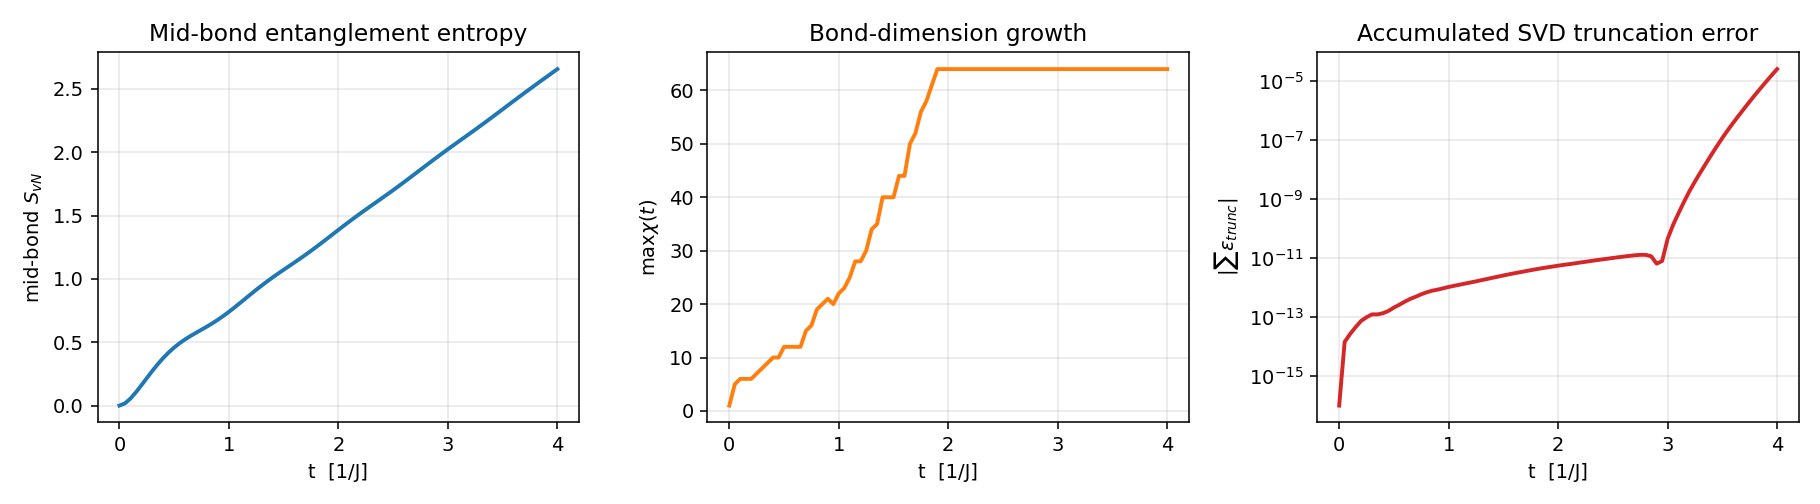
\includegraphics[width=0.88\linewidth]{summary.png}
  \caption{Reference $L=20$ TFIM quench ($J=g=1$, order 4, $\chi_{\max}=64$).  Entanglement growth drives bond-dimension growth, which sets the SVD sizes that dominate runtime.}
  \label{fig:summary}
\end{figure}

\begin{figure}[h]
  \centering
  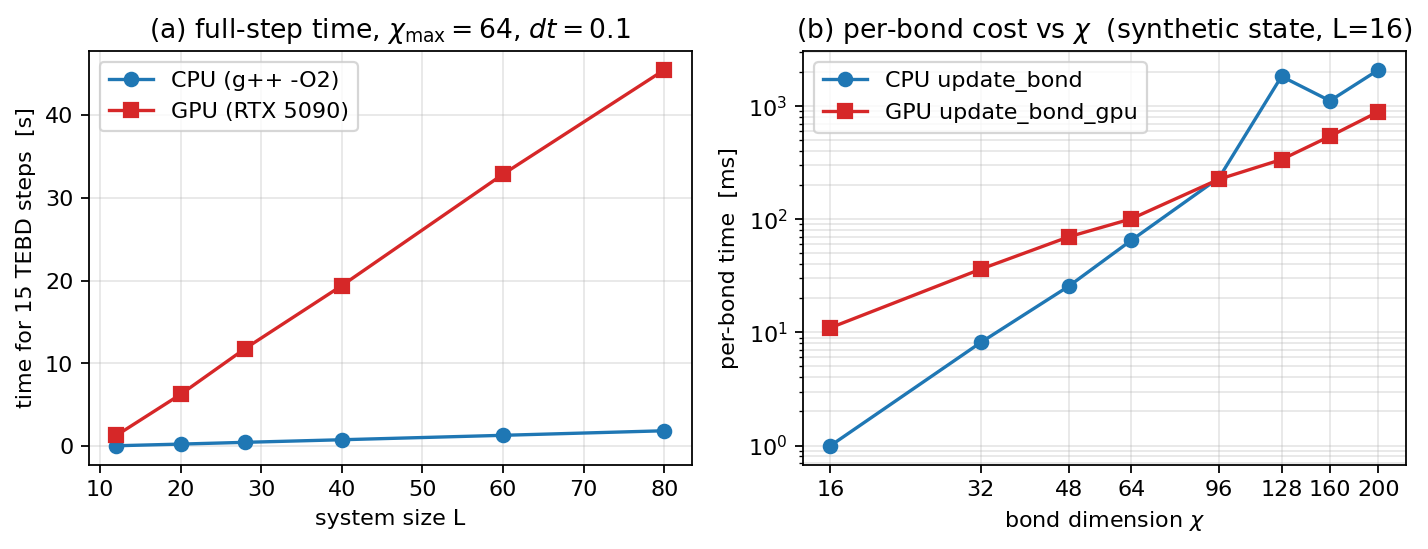
\includegraphics[width=0.88\linewidth]{bench_M3.png}
  \caption{(a) Wall time vs.\ $L$ at $\chi_{\max}=64$: linear, $\sim1.3$ ms/bond, latency-bound as predicted. (b) Per-call \code{update\_bond} vs.\ $\chi$: CPU/GPU crossover near $\chi\approx96$--128.}
  \label{fig:crossover}
\end{figure}

\begin{figure}[h]
  \centering
  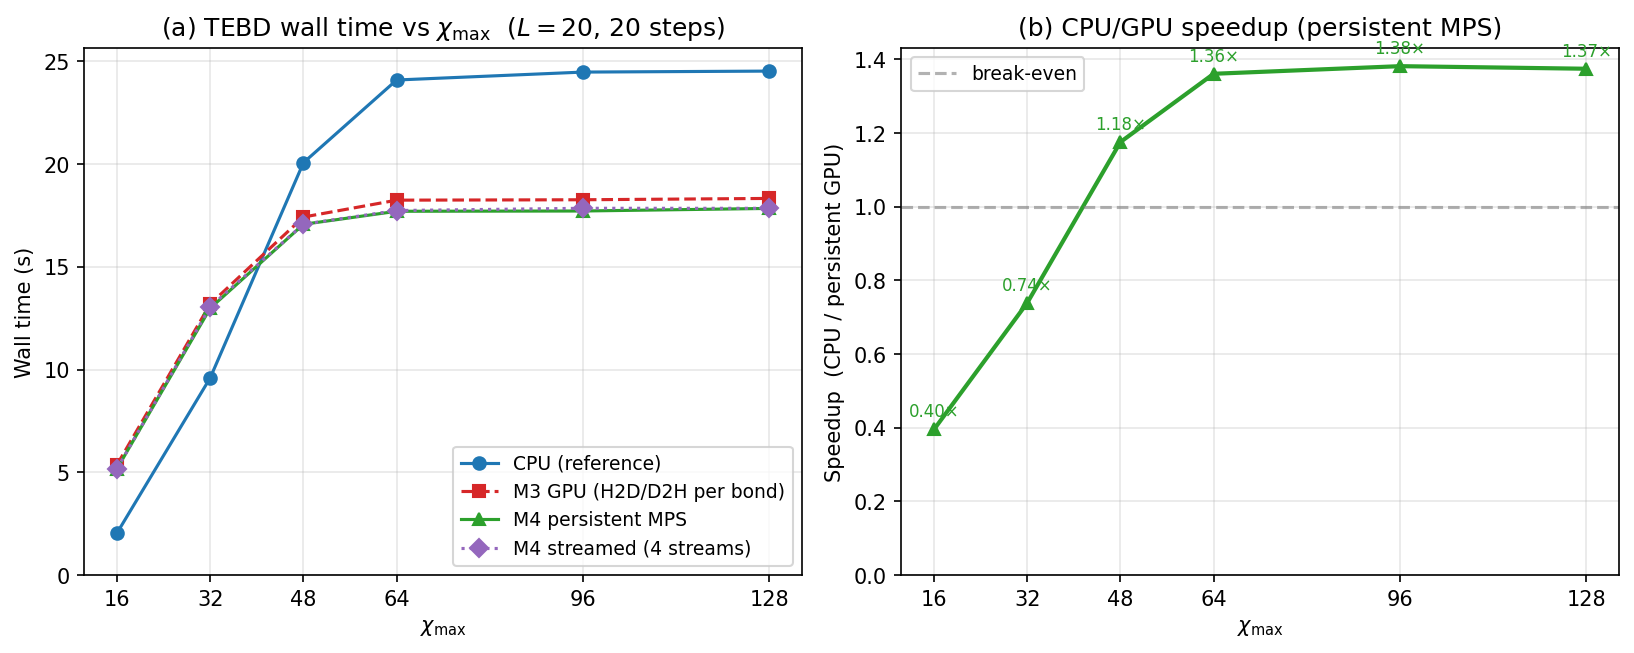
\includegraphics[width=0.72\linewidth]{m4_gpu_timing.png}
  \caption{Single-GPU full-step timing vs.\ $\chi_{\max}$ (companion to Table~\ref{tab:gpu}).}
  \label{fig:gputiming}
\end{figure}

\begin{figure}[h]
  \centering
  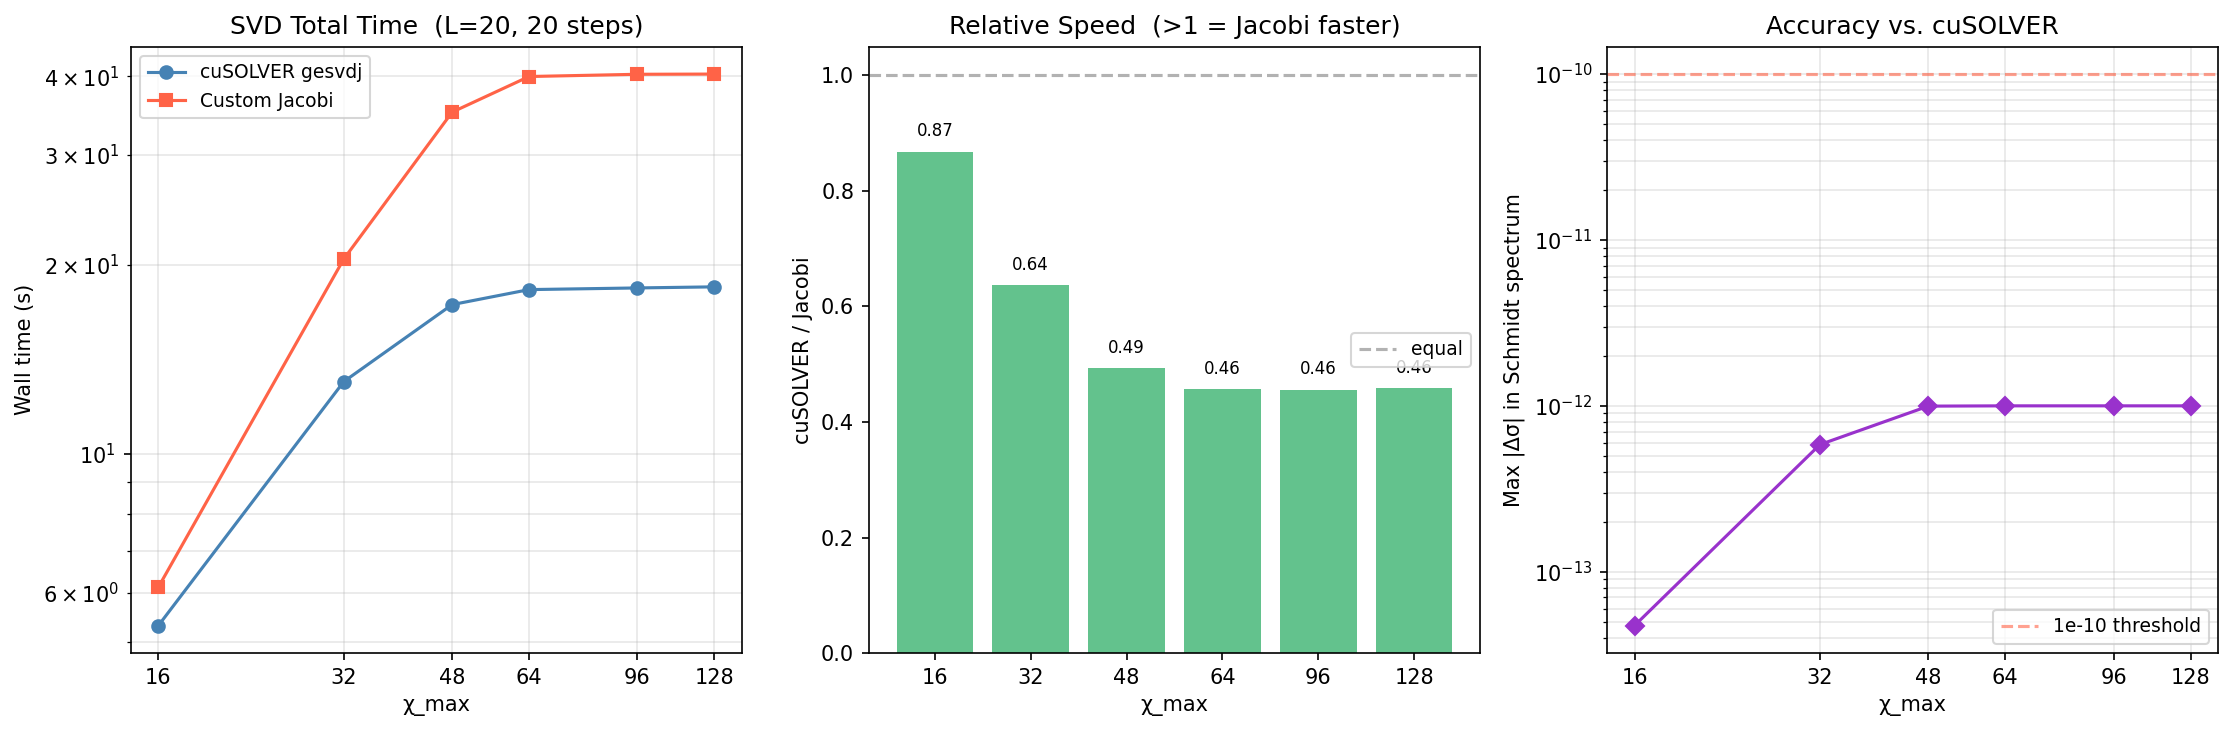
\includegraphics[width=0.92\linewidth]{svd_compare.png}
  \caption{Custom Jacobi SVD vs.\ cuSOLVER \code{gesvdj}: time ratio (center) and
  Schmidt-spectrum error (right). Both plateau above $\chi_{\max}=64$ (companion to Table~\ref{tab:svd}).}
  \label{fig:svd}
\end{figure}

\begin{figure}[h]
  \centering
  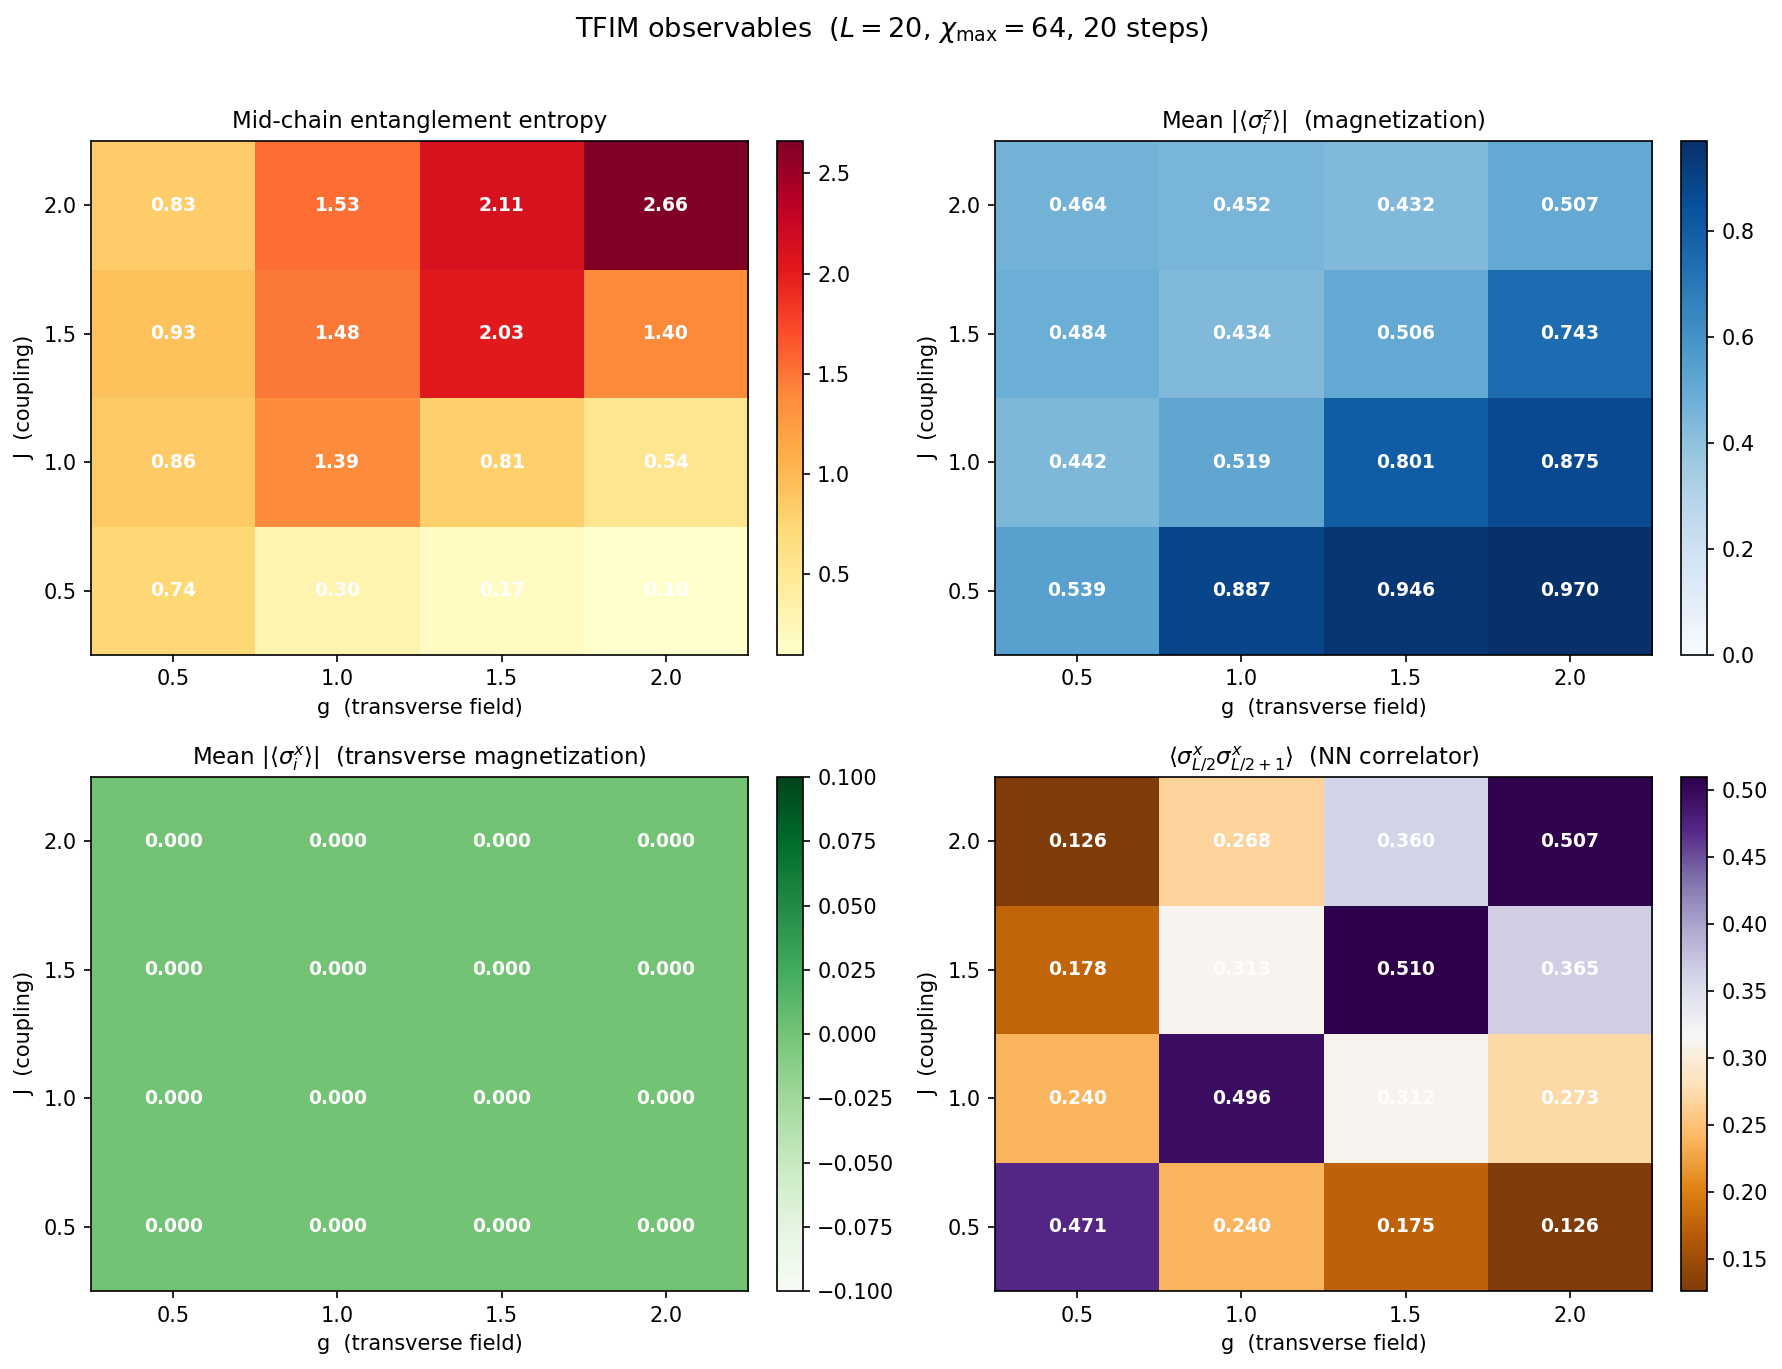
\includegraphics[width=0.92\linewidth]{observables_heatmap.png}
  \caption{GPU-computed observables over the $(J,g)$ phase diagram ($L=20$, $\chi_{\max}=64$, 20 Trotter steps at $dt=0.1$). Top-right: mean   $|\langle\sigma^z_i\rangle|$. Bottom-left: mean $|\langle\sigma^x_i\rangle|=0$   (zero by parity). Bottom-right: nearest-neighbour $x$-correlator.}
  \label{fig:obs}
\end{figure}

\begin{figure}[h]
  \centering
  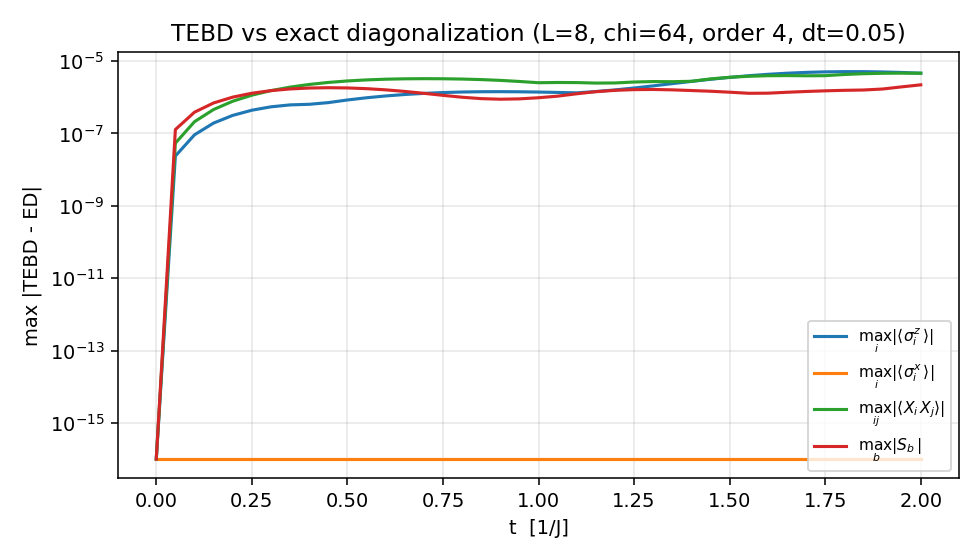
\includegraphics[width=0.72\linewidth]{validate_errors.png}
  \caption{TEBD vs.\ exact diagonalization, per-step max error. Final fidelity loss
  $4.3\times10^{-11}$.}
  \label{fig:validate}
\end{figure}

%% -------------------------------------------------------------------------
\section{Custom-kernel profile (Nsight Compute)}\label{app:ncu}

\noindent Nsight Compute (\code{ncu}) on the custom one-sided Jacobi kernel at $\chi_{\max}=128$ ($256\times256$ complex matrix, launched \code{<<<1,128>>>}):

\smallskip
\begin{center}\begin{tabular}{lrl}
\toprule
Metric & Value & Implication \\
\midrule
Compute (SM) throughput      & 0.42\%              & not compute-bound \\
DRAM throughput              & 0.00\% (10.8 MB/s)  & not bandwidth-bound \\
L2 / L1 hit rate             & $\approx$100\% / 92.6\% & matrix is cache-resident \\
Achieved occupancy           & 12.5\% (4/32 warps) & one block (not a resource cap) \\
SMs active                   & 1 of 72             & grid is a single block \\
Full waves across SMs        & 0.0                 & cannot fill one device wave \\
Warp cycles per issued inst. & 22.1                & long gaps between issues \\
Top stall (41.6\%)           & CTA barrier         & idle at \code{\_\_syncthreads} \\
Avg active threads/warp      & 29.2 (18.1 pred.)   & minor lane divergence \\
\bottomrule
\end{tabular}
\end{center}

\smallskip
\captionof{table}{The custom kernel is neither compute- nor memory-bound; it is under-decomposed and latency-bound. A single $128$-thread block uses $\approx0.17\%$ of the device ($12.5\%$ occupancy $\times$ 1/72 SMs), leaving the GPU $\approx99.8\%$ idle, with $41.6\%$ of stall cycles at \code{\_\_syncthreads}. The $12.5\%$ occupancy reflects the one-block grid, not a register or shared-memory cap (theoretical occupancy is $100\%$).}\label{tab:ncu}

\smallskip
\noindent\textbf{Why the barriers dominate.} The custom Jacobi SVD carries significant synchronization overhead. For each column-pair rotation, threads first compute partial dot products and norms, then reduce them in shared memory to obtain the rotation parameters; these reductions need \code{\_\_syncthreads()} barriers so that all partial sums are complete before the next reduction stage reads them. After one thread computes the rotation angle, another barrier is required before the rest of the block uses that angle to update the two columns. Since a sweep applies many such rotations sequentially and each small SVD exposes only a few warps of work, there is little independent work available to hide the barrier latency.



\newpage
\section*{References}

\begin{enumerate}
\item G. Vidal, \emph{Efficient classical simulation of slightly entangled quantum
  computations}, PRL 91, 147902 (2003); \emph{Efficient simulation of one-dimensional
  quantum many-body systems}, PRL 93, 040502 (2004).
\item U. Schollw{\"o}ck, \emph{The density-matrix renormalization group in the age of matrix
  product states}, Ann.\ Phys.\ 326, 96 (2011).
\item R.\,P. Brent and F.\,T. Luk, \emph{The solution of singular-value and symmetric
  eigenvalue problems on multiprocessor arrays}, SIAM J.\ Sci.\ Stat.\ Comput.\ (1985).
\item N. Hatano and M. Suzuki, \emph{Finding exponential product formulas of higher
  orders} (Suzuki--Trotter decomposition).
\item NVIDIA cuSOLVER / cuQuantum (cuTensorNet) documentation.
\item TeNPy, ITensor, quimb (open-source tensor-network libraries).
\end{enumerate}

\end{document}
